\documentclass{beamer}
\usetheme{metropolis}


\title{DevClub: Cloud Native Infrastructure: Container in Deatil}
\date{\today}

\title{Cloud Native Introduction: Docker and K8s}

\begin{document}
    \maketitle
    \begin{frame}{Docker In Detail}
        \begin{itemize}

            \item Container
            \begin{itemize}
                \item Infrastructure of Isolation: Namespace 
                \item Resource Limit: CGroup
                \item Image System:  OverlayFS
                \item Docker Container Network
                \item GPU Support: Nvidia Container Runtime(NVCR)
                \item[$\square$] Practice: Container without Docker
                \item[$\square$] Real Case: Uasge in PTM LeaderBoard
            \end{itemize}

            \item Orchestration ()
            \begin{itemize}
                \item Workload Resources - beyond the single container
                \item Network - how to expose service
                \item Storage - model and taxonomy
                \item[$\square$] Practice: deploy a simple service
            \end{itemize}

        \end{itemize}
    \end{frame}
    \begin{frame}{Infrastructure of Isolation: Namespace }
    \begin{itemize}
        \item A namespace wraps a global system resource.
        \pause
        \item System resource can be: cgroup,IPC,Network,Mount,PID,Time,User,TS
        \pause
        \item A process belongs to one specific namespace, and can only see resource tagged with same namespace.
    \end{itemize}
    \pause
    \begin{columns}
        \begin{column}{0.7\textwidth}
            \begin{figure}
                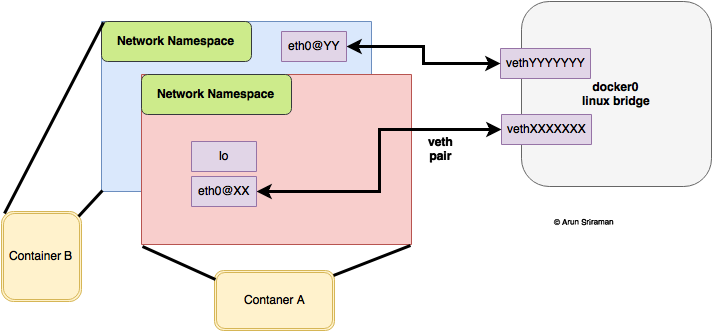
\includegraphics[width=1\textwidth]{assets/network.png}
                \caption{docker network isolation }
            \end{figure}
        \end{column}
        \begin{column}{0.3\textwidth}
            Let's take \textbf{netns} as example.
        \end{column}
    \end{columns}
\end{frame}
    \begin{frame}{Resource Limit: cgroups}
    \begin{itemize}
        \item cgroups can \textbf{limit, account, priorizate} resource usage of a collection of processes.
        \pause
        \item resource usage can be: CPU Time, memory, disk I/O, network.
        \pause
        \item We can use cgroup\textbf{fs} to interact with cgroup.
    \end{itemize}
    
    \pause
            \begin{figure}
        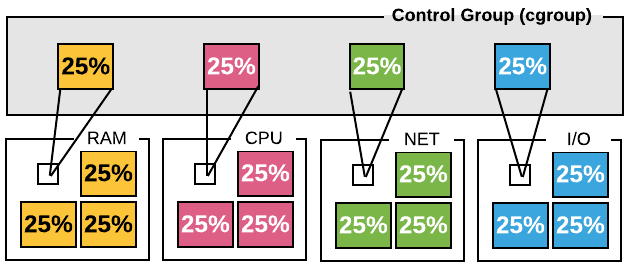
\includegraphics[width=.8\textwidth]{assets/cgroup.png}
                \caption{cgroup usage}

            \end{figure}
\end{frame}
    \begin{frame}{Image System:  OverlayFS}
    \begin{itemize}
        \item OverlayFS is a union mount filesystem implementation.
        \pause
        \item We can use it combine multiple directories.
        \pause
        \item The dokcer build system is built on this feature.
    \end{itemize}

    \begin{columns}
        \begin{column}{0.7\textwidth}
            \begin{figure}
                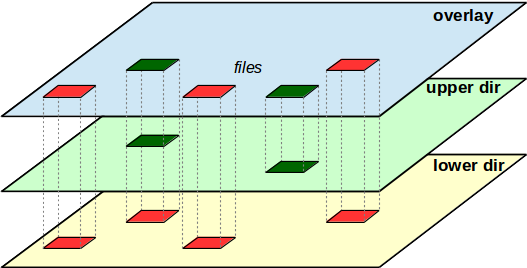
\includegraphics[width=1\textwidth]{assets/overlayfs.png}
                \caption{Overlayfs Diagram}
            \end{figure}
        \end{column}
        \begin{column}{0.3\textwidth}
            Let's practice overlayfs in real system
        \end{column}
    \end{columns}
\end{frame}
    \begin{frame}{Docker Container Network}
In \textbf{docker}, we mainly use four kinds of network.
    \begin{itemize}
        \pause
        \item \textbf{Bridge}: A Bridge Network provide network isolation.
        \pause
        \item \textbf{Overlay}: Overlay Network provide connectivity between different containers.
        \pause
        \item \textbf{Host}: Host Network remove network isolation between the container and the Docker host
        \pause
        \item \textbf{MacVlan}: MacVlan assign a MAC address to container which makes the container looks like a real node.
    \end{itemize}

\end{frame}
    \begin{frame}{GPU Support: Nvidia Container Runtime(NVCR)}
    \begin{columns}
        \begin{column}{0.7\textwidth}
            \begin{figure}
                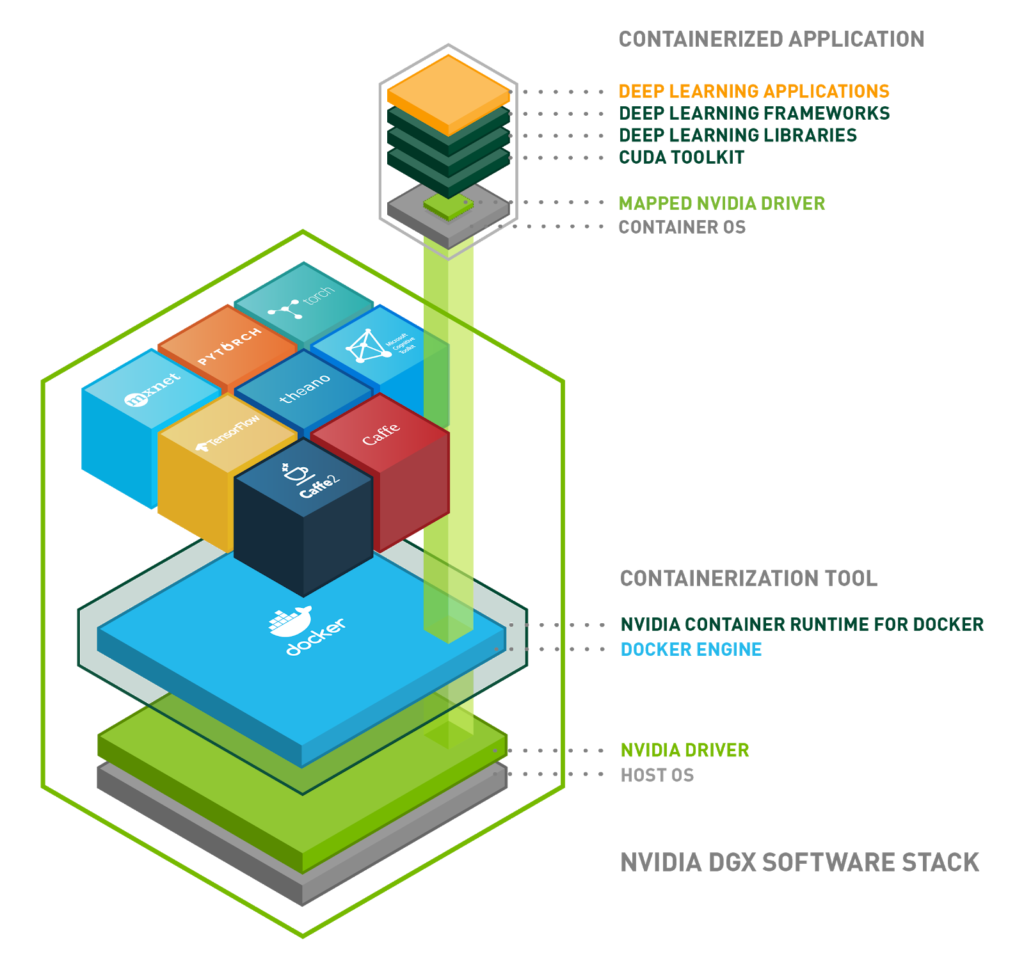
\includegraphics[width=1\textwidth]{assets/dgx-docker-1024x970.png}
                \caption{Nvidia-Docker diagram}
            \end{figure}
        \end{column}
        \begin{column}{0.5\textwidth}
            \pause
            nvidia docker is composed with 
            \begin{itemize}
                \item nvidia-docker 
                \item nvidia-container-runtime
                \item libnvidia-container
            \end{itemize}

            \pause
            Those three components are equivalent to

            \begin{itemize}
                \item docker
                \item runC
                \item libcontainer
            \end{itemize}


        \end{column}
    \end{columns}
\end{frame}

\end{document}